\section{Motivation}

\frame{
	\frametitle{}
	\begin{figure}
	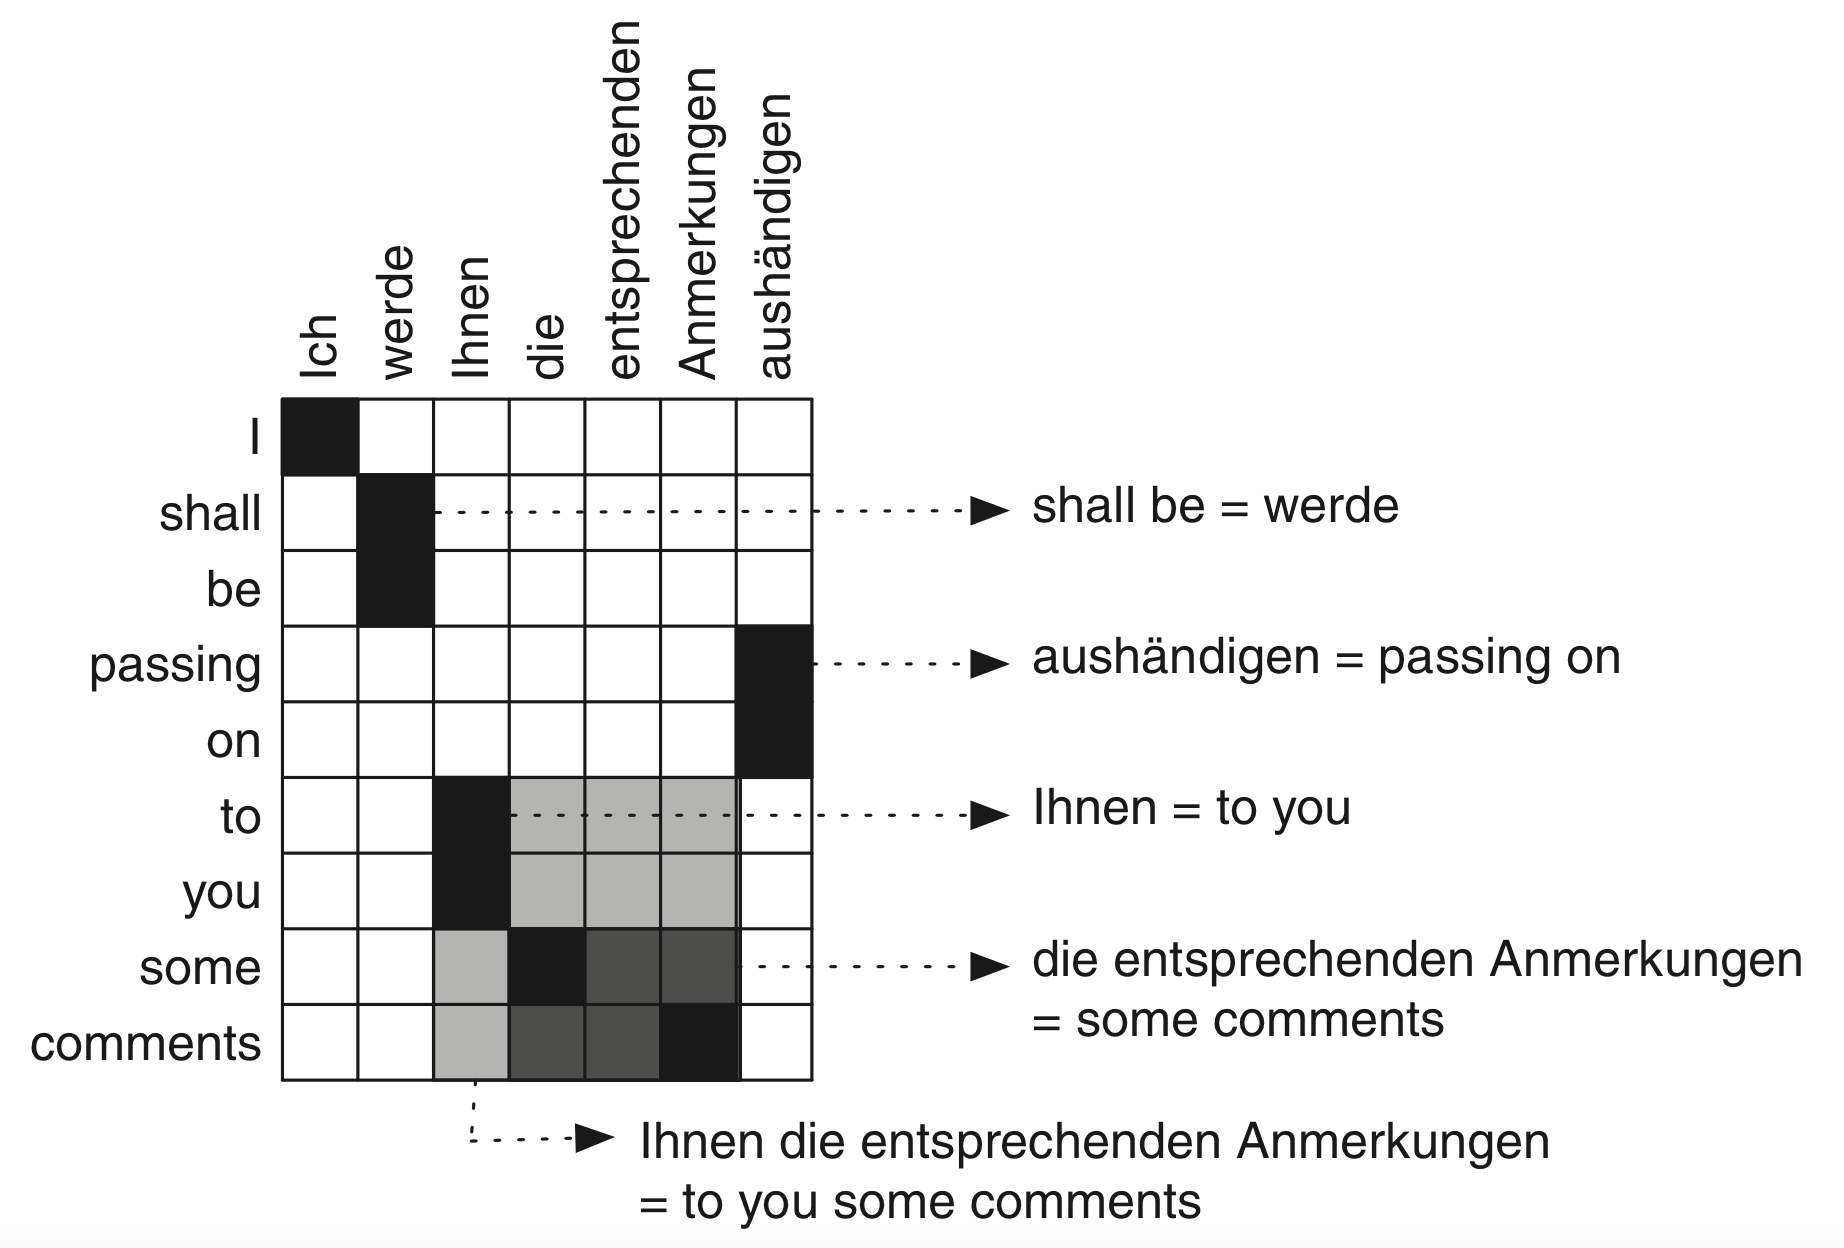
\includegraphics[scale=0.25]{img/motivation}
	\caption{\citet{Koehn:2010:SMT}}
	\end{figure}
	
	$$\ftext{werde } X \ftext{ aush\"andigen } | \etext{ shall be passing on } X $$
}


\frame{
	\frametitle{Why hierarchical structure?}
	
	Better generalisation
	\begin{itemize}
		\item compositionality
		\item reordering
	\end{itemize}
}

\frame{
	\frametitle{Why is reordering important?}
	
	Monotone translation is unrealistic
	\begin{itemize}
		\item languages differ wrt word-order\\ \pause
		e.g. different syntactic structure\\ \pause
		e.g. rich morphology \pause
	\end{itemize}

	~
	
	Reordering is arguably one of the hardest problems in MT \pause
	\begin{itemize}
		\item part of the model of translational equivalences\\
		\emph{the part that determines the space of translations}
	\end{itemize}
	
}

\frame{
	\frametitle{Key aspects}	
	
	Expressiveness
	\begin{itemize}
		\item how much can two languages differ wrt word order?
	\end{itemize}
	
	\pause
	
	Modelling
	\begin{itemize}
		\item how many parameters do we have to estimate?
	\end{itemize}

}